\documentclass[]{article}
\usepackage{lmodern}
\usepackage{amssymb,amsmath}
\usepackage{ifxetex,ifluatex}
\usepackage{fixltx2e} % provides \textsubscript
\ifnum 0\ifxetex 1\fi\ifluatex 1\fi=0 % if pdftex
  \usepackage[T1]{fontenc}
  \usepackage[utf8]{inputenc}
\else % if luatex or xelatex
  \ifxetex
    \usepackage{mathspec}
  \else
    \usepackage{fontspec}
  \fi
  \defaultfontfeatures{Ligatures=TeX,Scale=MatchLowercase}
\fi
% use upquote if available, for straight quotes in verbatim environments
\IfFileExists{upquote.sty}{\usepackage{upquote}}{}
% use microtype if available
\IfFileExists{microtype.sty}{%
\usepackage[]{microtype}
\UseMicrotypeSet[protrusion]{basicmath} % disable protrusion for tt fonts
}{}
\PassOptionsToPackage{hyphens}{url} % url is loaded by hyperref
\usepackage[unicode=true]{hyperref}
\hypersetup{
            pdftitle={Summary of Genicot and Ray (2017): Aspirations and Inequality},
            pdfauthor={Nick Hoffman},
            pdfborder={0 0 0},
            breaklinks=true}
\urlstyle{same}  % don't use monospace font for urls
\usepackage[margin=1in]{geometry}
\usepackage{color}
\usepackage{fancyvrb}
\newcommand{\VerbBar}{|}
\newcommand{\VERB}{\Verb[commandchars=\\\{\}]}
\DefineVerbatimEnvironment{Highlighting}{Verbatim}{commandchars=\\\{\}}
% Add ',fontsize=\small' for more characters per line
\usepackage{framed}
\definecolor{shadecolor}{RGB}{248,248,248}
\newenvironment{Shaded}{\begin{snugshade}}{\end{snugshade}}
\newcommand{\KeywordTok}[1]{\textcolor[rgb]{0.13,0.29,0.53}{\textbf{#1}}}
\newcommand{\DataTypeTok}[1]{\textcolor[rgb]{0.13,0.29,0.53}{#1}}
\newcommand{\DecValTok}[1]{\textcolor[rgb]{0.00,0.00,0.81}{#1}}
\newcommand{\BaseNTok}[1]{\textcolor[rgb]{0.00,0.00,0.81}{#1}}
\newcommand{\FloatTok}[1]{\textcolor[rgb]{0.00,0.00,0.81}{#1}}
\newcommand{\ConstantTok}[1]{\textcolor[rgb]{0.00,0.00,0.00}{#1}}
\newcommand{\CharTok}[1]{\textcolor[rgb]{0.31,0.60,0.02}{#1}}
\newcommand{\SpecialCharTok}[1]{\textcolor[rgb]{0.00,0.00,0.00}{#1}}
\newcommand{\StringTok}[1]{\textcolor[rgb]{0.31,0.60,0.02}{#1}}
\newcommand{\VerbatimStringTok}[1]{\textcolor[rgb]{0.31,0.60,0.02}{#1}}
\newcommand{\SpecialStringTok}[1]{\textcolor[rgb]{0.31,0.60,0.02}{#1}}
\newcommand{\ImportTok}[1]{#1}
\newcommand{\CommentTok}[1]{\textcolor[rgb]{0.56,0.35,0.01}{\textit{#1}}}
\newcommand{\DocumentationTok}[1]{\textcolor[rgb]{0.56,0.35,0.01}{\textbf{\textit{#1}}}}
\newcommand{\AnnotationTok}[1]{\textcolor[rgb]{0.56,0.35,0.01}{\textbf{\textit{#1}}}}
\newcommand{\CommentVarTok}[1]{\textcolor[rgb]{0.56,0.35,0.01}{\textbf{\textit{#1}}}}
\newcommand{\OtherTok}[1]{\textcolor[rgb]{0.56,0.35,0.01}{#1}}
\newcommand{\FunctionTok}[1]{\textcolor[rgb]{0.00,0.00,0.00}{#1}}
\newcommand{\VariableTok}[1]{\textcolor[rgb]{0.00,0.00,0.00}{#1}}
\newcommand{\ControlFlowTok}[1]{\textcolor[rgb]{0.13,0.29,0.53}{\textbf{#1}}}
\newcommand{\OperatorTok}[1]{\textcolor[rgb]{0.81,0.36,0.00}{\textbf{#1}}}
\newcommand{\BuiltInTok}[1]{#1}
\newcommand{\ExtensionTok}[1]{#1}
\newcommand{\PreprocessorTok}[1]{\textcolor[rgb]{0.56,0.35,0.01}{\textit{#1}}}
\newcommand{\AttributeTok}[1]{\textcolor[rgb]{0.77,0.63,0.00}{#1}}
\newcommand{\RegionMarkerTok}[1]{#1}
\newcommand{\InformationTok}[1]{\textcolor[rgb]{0.56,0.35,0.01}{\textbf{\textit{#1}}}}
\newcommand{\WarningTok}[1]{\textcolor[rgb]{0.56,0.35,0.01}{\textbf{\textit{#1}}}}
\newcommand{\AlertTok}[1]{\textcolor[rgb]{0.94,0.16,0.16}{#1}}
\newcommand{\ErrorTok}[1]{\textcolor[rgb]{0.64,0.00,0.00}{\textbf{#1}}}
\newcommand{\NormalTok}[1]{#1}
\usepackage{graphicx,grffile}
\makeatletter
\def\maxwidth{\ifdim\Gin@nat@width>\linewidth\linewidth\else\Gin@nat@width\fi}
\def\maxheight{\ifdim\Gin@nat@height>\textheight\textheight\else\Gin@nat@height\fi}
\makeatother
% Scale images if necessary, so that they will not overflow the page
% margins by default, and it is still possible to overwrite the defaults
% using explicit options in \includegraphics[width, height, ...]{}
\setkeys{Gin}{width=\maxwidth,height=\maxheight,keepaspectratio}
\IfFileExists{parskip.sty}{%
\usepackage{parskip}
}{% else
\setlength{\parindent}{0pt}
\setlength{\parskip}{6pt plus 2pt minus 1pt}
}
\setlength{\emergencystretch}{3em}  % prevent overfull lines
\providecommand{\tightlist}{%
  \setlength{\itemsep}{0pt}\setlength{\parskip}{0pt}}
\setcounter{secnumdepth}{0}
% Redefines (sub)paragraphs to behave more like sections
\ifx\paragraph\undefined\else
\let\oldparagraph\paragraph
\renewcommand{\paragraph}[1]{\oldparagraph{#1}\mbox{}}
\fi
\ifx\subparagraph\undefined\else
\let\oldsubparagraph\subparagraph
\renewcommand{\subparagraph}[1]{\oldsubparagraph{#1}\mbox{}}
\fi

% set default figure placement to htbp
\makeatletter
\def\fps@figure{htbp}
\makeatother


\title{Summary of Genicot and Ray (2017): Aspirations and Inequality}
\author{Nick Hoffman}
\date{March 19, 2020}

\begin{document}
\maketitle

\subsection{Introduction}\label{introduction}

\begin{itemize}
\tightlist
\item
  What role do ``aspirations'' play in generating growth and income
  inequality?
\item
  Three questions

  \begin{enumerate}
  \def\labelenumi{\arabic{enumi}.}
  \tightlist
  \item
    How do individuals \emph{form} aspirations?
  \item
    How do individuals \emph{react to} aspirations?
  \item
    How does the behavior of individuals, with reference to aspirations,
    aggregate?
  \end{enumerate}
\item
  How the authors address these questions

  \begin{enumerate}
  \def\labelenumi{\arabic{enumi}.}
  \tightlist
  \item
    Aspirations take the form of endogeneous thresholds in the utility
    function, influenced by individual income and society-wide
    distribution
  \item
    Crossing one of these thresholds generates ``bonus'' utility
  \item
    This theory is embedded into an A-K model of growth
  \end{enumerate}
\item
  Interaction between aspirations and inequality: two environments

  \begin{enumerate}
  \def\labelenumi{\arabic{enumi}.}
  \tightlist
  \item
    Bounded incomes: steady-state aspirations, no perfect equality
  \item
    Sustained growth: intitial conditions determine asymptotic behavior

    \begin{itemize}
    \tightlist
    \item
      If initial distribution is relatively equal, incomes converge to
      BGP
    \item
      If initial distribution is unequal, income growth rates will
      \emph{cluster}, leading to forever-increasing inequality
    \end{itemize}
  \end{enumerate}
\end{itemize}

\subsection{Model}\label{model}

\subsubsection{Agents and Payoffs}\label{agents-and-payoffs}

A parent-child pair makes up a dynasty. The parent allocates lifetime
income \(y\) between consumption \(c\) and investment in child's wealth
\(z\). The payoff to the parent is: \[u(c) + w_0(z) + w_1(e)\] where
\(w_0\) is the intrinsic parental utility from the child's wealth, and
\(w_1\) the milestone utility from passing a threshold \(a\), with
\(e = \max\{z - a, 0\}\).

For the purposes of recreating the figures in the paper, I use the
specification that the authors use in their examples. Namely,

\begin{align}
    u(c) &= c^{1 - \sigma} & w_0(z) &= \delta z^{1 - \sigma} & w_1(e) &= \delta \pi e^{1 - \sigma}
\end{align}

with \(\sigma = 0.65\), discount factor \(\delta = 0.95\), and
\(\pi = 1.1\) the ``bonus'' utility attained by crossing the threshold
\(a\).

The following plot shows the payoff as a function of \(z\) and \(a\).
Here, I set \(a\) equal to 1:

\begin{Shaded}
\begin{Highlighting}[]
\CommentTok{# Parameters}
\NormalTok{sig <-}\StringTok{ }\FloatTok{0.65}
\NormalTok{del <-}\StringTok{ }\FloatTok{0.95}
\NormalTok{pi <-}\StringTok{ }\FloatTok{1.1}

\CommentTok{# Payoff functions}
\NormalTok{util <-}\StringTok{ }\ControlFlowTok{function}\NormalTok{(c) \{c }\OperatorTok{^}\StringTok{ }\NormalTok{(}\DecValTok{1} \OperatorTok{-}\StringTok{ }\NormalTok{sig)\}}
\NormalTok{w0 <-}\StringTok{ }\ControlFlowTok{function}\NormalTok{(z) \{del }\OperatorTok{*}\StringTok{ }\NormalTok{z }\OperatorTok{^}\StringTok{ }\NormalTok{(}\DecValTok{1} \OperatorTok{-}\StringTok{ }\NormalTok{sig)\}}
\NormalTok{w1 <-}\StringTok{ }\ControlFlowTok{function}\NormalTok{(e) \{del }\OperatorTok{*}\StringTok{ }\NormalTok{pi }\OperatorTok{*}\StringTok{ }\NormalTok{e }\OperatorTok{^}\StringTok{ }\NormalTok{(}\DecValTok{1} \OperatorTok{-}\StringTok{ }\NormalTok{sig)\}}
\NormalTok{fig1_payoff <-}\StringTok{ }\ControlFlowTok{function}\NormalTok{(z, a) \{}
  \KeywordTok{w0}\NormalTok{(z) }\OperatorTok{+}\StringTok{ }\KeywordTok{w1}\NormalTok{(}\KeywordTok{max}\NormalTok{(}\KeywordTok{c}\NormalTok{(z }\OperatorTok{-}\StringTok{ }\NormalTok{a, }\DecValTok{0}\NormalTok{)))}
\NormalTok{\}}
\NormalTok{fig1_payoff <-}\StringTok{ }\KeywordTok{Vectorize}\NormalTok{(fig1_payoff, }\DataTypeTok{vectorize.args =} \StringTok{"z"}\NormalTok{)}
\end{Highlighting}
\end{Shaded}

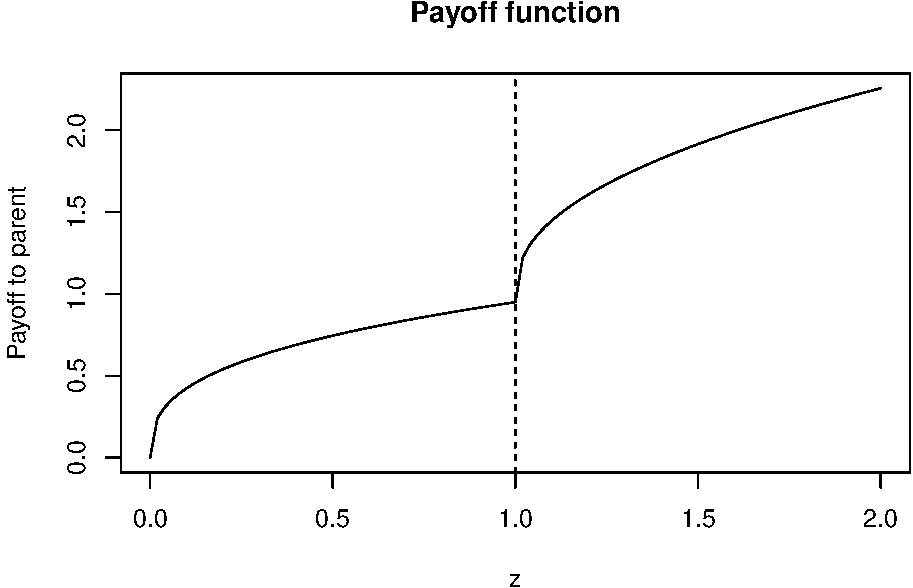
\includegraphics{genicot_ray_notes_files/figure-latex/unnamed-chunk-1-1.pdf}
The jump at \(a = 1\) represents the bonus payoff. A change in the level
of aspirations will move this ``kink'' point to the left or right.

\subsubsection{Formation of Aspirations}\label{formation-of-aspirations}

The authors assume a flexible format for the aspiration-generating
function: \[a = \Psi(y,F)\] where \(y\) is an individual's income and
\(F\) is the society-wide distribution of incomes. They place the
following assumptions on \(\Psi\):

\begin{itemize}
\tightlist
\item
  Regularity: \(\Psi\) is continuous and nondecreasing in \(y\).
\item
  Scale invariance: \(\Psi(\lambda y, F^\lambda) = \lambda\Psi(y, F)\)
\item
  Range-boundedness:
  \(\min\{y, \min F\} \leq \Psi(y, F) \leq \max(y, \max F)\)
\item
  Social monotonicity: \(\forall y\),
  \(\Psi(y,F) \leq \Psi(y, F^\prime)\) if \(F \leq F^\prime\) in the
  sense of first-order stochasic dominance.
\end{itemize}

\subsubsection{Consumption-Savings Decision with
Aspirations}\label{consumption-savings-decision-with-aspirations}

To formalize the problem of a representative parent in this model,
define \(f(k) = \rho k\), the production function that turns investment
\(k\) into next-period wealth. Let \(k(z) = f^{-1}(z)\) be the inverse,
which maps desired next-period wealth into current investment. The
parent's problem is now
\[\max_z u(y - k(z)) + w_0(z) + w_1(\max\{z - a, 0\})\] I again use the
authors' example, where \(f(k) = \rho k\), with \(\rho > 1\).

The chart below illustrates this graphically, following Figure 3 in the
paper:

\begin{Shaded}
\begin{Highlighting}[]
\NormalTok{rho <-}\StringTok{ }\FloatTok{1.01}
\NormalTok{prod <-}\StringTok{ }\ControlFlowTok{function}\NormalTok{(z) rho }\OperatorTok{*}\StringTok{ }\NormalTok{z}
\NormalTok{finv <-}\StringTok{ }\ControlFlowTok{function}\NormalTok{(z) z }\OperatorTok{/}\StringTok{ }\NormalTok{rho }\CommentTok{# called 'k' in the paper}
\NormalTok{fig2_cost <-}\StringTok{ }\ControlFlowTok{function}\NormalTok{(y, z)\{}
  \KeywordTok{util}\NormalTok{(y) }\OperatorTok{-}\StringTok{ }\KeywordTok{util}\NormalTok{(y }\OperatorTok{-}\StringTok{ }\KeywordTok{finv}\NormalTok{(z))}
\NormalTok{\}}
\NormalTok{fig2_cost <-}\StringTok{ }\KeywordTok{Vectorize}\NormalTok{(fig2_cost, }\DataTypeTok{vectorize.args =} \StringTok{"z"}\NormalTok{)}
\end{Highlighting}
\end{Shaded}

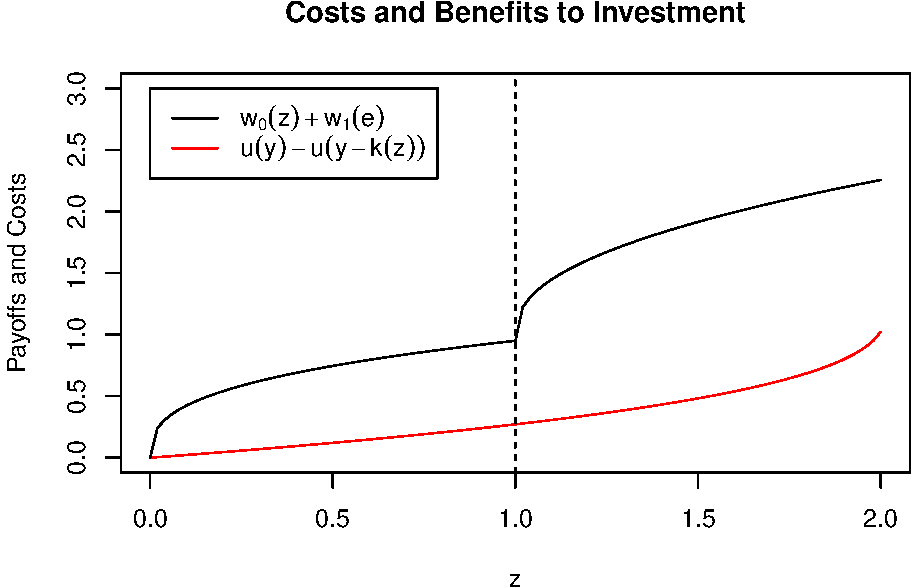
\includegraphics{genicot_ray_notes_files/figure-latex/unnamed-chunk-2-1.pdf}

The red black line shows the payoff to investment \(z\) (with \(a= 1\)),
while the red line shows the cost, relative to consuming all of one's
income. The objective, then, is to maximize the distance between these
two. Because of the concavity of both functions, there will be at most
two local maxima of this distance: one to the left of \(a\), and one to
the right. The authors refer to these points as \(z_0\) and \(z_1\),
respectively. Finding these amounts to solving two first order
conditions:
\[w_0^\prime(z_0) = \frac{u^\prime(y - k(z_0))}{f^\prime(k(z_0))}\] and
\[w_0^\prime(z_1) + w_1^\prime(z_1 - a) = \frac{u^\prime(y - k(z_1))}{f^\prime(k(z_1))}\]

The parent then chooses whichever \(z\) among these two leads to a
higher payoff. The following code solves for \(z_0\) and \(z_1\) as a
function of \(a\):

\begin{Shaded}
\begin{Highlighting}[]
\CommentTok{# Derivatives}
\NormalTok{util_p <-}\StringTok{ }\ControlFlowTok{function}\NormalTok{(c) \{(}\DecValTok{1} \OperatorTok{-}\StringTok{ }\NormalTok{sig) }\OperatorTok{*}\StringTok{ }\NormalTok{c }\OperatorTok{^}\StringTok{ }\OperatorTok{-}\NormalTok{sig\}}
\NormalTok{w0_p <-}\StringTok{ }\ControlFlowTok{function}\NormalTok{(z) \{del }\OperatorTok{*}\StringTok{ }\NormalTok{(}\DecValTok{1} \OperatorTok{-}\StringTok{ }\NormalTok{sig) }\OperatorTok{*}\StringTok{ }\NormalTok{z }\OperatorTok{^}\StringTok{ }\OperatorTok{-}\NormalTok{sig\}}
\NormalTok{w1_p <-}\StringTok{ }\ControlFlowTok{function}\NormalTok{(e) \{del }\OperatorTok{*}\StringTok{ }\NormalTok{pi }\OperatorTok{*}\StringTok{ }\NormalTok{(}\DecValTok{1} \OperatorTok{-}\StringTok{ }\NormalTok{sig) }\OperatorTok{*}\StringTok{ }\NormalTok{e }\OperatorTok{^}\StringTok{ }\OperatorTok{-}\NormalTok{sig\}}

\NormalTok{zopt0 <-}\StringTok{ }\ControlFlowTok{function}\NormalTok{(z, y) \{ }\CommentTok{# z < a}
  \KeywordTok{w0_p}\NormalTok{(z) }\OperatorTok{-}\StringTok{ }\NormalTok{(}\KeywordTok{util_p}\NormalTok{(y }\OperatorTok{-}\StringTok{ }\KeywordTok{finv}\NormalTok{(z)) }\OperatorTok{/}\StringTok{ }\NormalTok{rho)}
\NormalTok{\}}
\NormalTok{zopt0 <-}\StringTok{ }\KeywordTok{Vectorize}\NormalTok{(zopt0, }\DataTypeTok{vectorize.args =} \StringTok{"z"}\NormalTok{)}

\NormalTok{zopt1 <-}\StringTok{ }\ControlFlowTok{function}\NormalTok{(z, y, a) \{ }\CommentTok{# z > a}
  \KeywordTok{w0_p}\NormalTok{(z) }\OperatorTok{+}\StringTok{ }\KeywordTok{w1_p}\NormalTok{(z }\OperatorTok{-}\StringTok{ }\NormalTok{a) }\OperatorTok{-}\StringTok{ }\NormalTok{(}\KeywordTok{util_p}\NormalTok{(y }\OperatorTok{-}\StringTok{ }\KeywordTok{finv}\NormalTok{(z)) }\OperatorTok{/}\StringTok{ }\NormalTok{rho)}
\NormalTok{\}}
\NormalTok{zopt1 <-}\StringTok{ }\KeywordTok{Vectorize}\NormalTok{(zopt1, }\DataTypeTok{vectorize.args =} \StringTok{"z"}\NormalTok{)}

\NormalTok{find_z <-}\StringTok{ }\ControlFlowTok{function}\NormalTok{(z, y, a)\{}
  \CommentTok{# Find the roots}
\NormalTok{  z0 =}\StringTok{ }\KeywordTok{uniroot}\NormalTok{(zopt0, }\DataTypeTok{interval =} \KeywordTok{c}\NormalTok{(}\DecValTok{0}\NormalTok{, }\DecValTok{2}\NormalTok{), }\DataTypeTok{y =}\NormalTok{ y, }\DataTypeTok{extendInt =} \StringTok{"yes"}\NormalTok{)}\OperatorTok{$}\NormalTok{root}
\NormalTok{  z1 =}\StringTok{ }\KeywordTok{uniroot}\NormalTok{(zopt1, }\DataTypeTok{interval =} \KeywordTok{c}\NormalTok{(}\FloatTok{1.5}\NormalTok{, }\FloatTok{1.6}\NormalTok{), }\DataTypeTok{y =}\NormalTok{ y, }\DataTypeTok{a =}\NormalTok{ a, }\DataTypeTok{extendInt =} \StringTok{"yes"}\NormalTok{)}\OperatorTok{$}\NormalTok{root}
  
  \CommentTok{# Which is better?}
\NormalTok{  u0 =}\StringTok{ }\KeywordTok{util}\NormalTok{(y }\OperatorTok{-}\StringTok{ }\KeywordTok{finv}\NormalTok{(z0)) }\OperatorTok{+}\StringTok{ }\KeywordTok{w0}\NormalTok{(z0)}
\NormalTok{  u1 =}\StringTok{ }\KeywordTok{util}\NormalTok{(y }\OperatorTok{-}\StringTok{ }\KeywordTok{finv}\NormalTok{(z1)) }\OperatorTok{+}\StringTok{ }\KeywordTok{w0}\NormalTok{(z0) }\OperatorTok{+}\StringTok{ }\KeywordTok{w1}\NormalTok{(}\KeywordTok{max}\NormalTok{(}\KeywordTok{c}\NormalTok{(z0 }\OperatorTok{-}\StringTok{ }\NormalTok{a, }\DecValTok{0}\NormalTok{)))}
  
  \ControlFlowTok{if}\NormalTok{ (u0 }\OperatorTok{>}\StringTok{ }\NormalTok{u1) \{}
    \KeywordTok{return}\NormalTok{(z0)}
\NormalTok{  \} }\ControlFlowTok{else}\NormalTok{ \{}
    \KeywordTok{return}\NormalTok{(z1)}
\NormalTok{  \}}
\NormalTok{\}}
\end{Highlighting}
\end{Shaded}

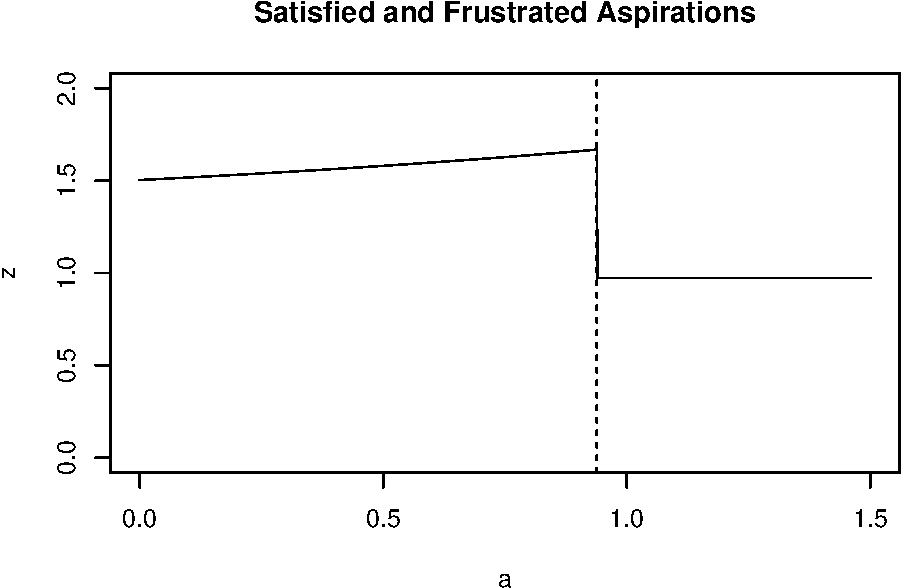
\includegraphics{genicot_ray_notes_files/figure-latex/unnamed-chunk-3-1.pdf}

The chart matches Figure 3 in the paper. The authors demonstrate that,
up to a threshold \(a^*\), aspirations will be \emph{satisfied}; that
is, the chosen \(z\) will be greater than aspirations \(a\). For
aspirations \(a>a^*\), however, aspirations will be \emph{frustrated},
with \(z<a\). Note that above \(a^*\), chosen wealth is insensitive to
aspirations. This feature of the model will lead to divergence in
growth, between those whose aspirations are frustrated and those whose
are satisfied.\footnote{The authors also discuss an extension in which
  investment \emph{declines} in aspirations when aspirations are
  frustrated.}

\subsection{Aspirations and Growth}\label{aspirations-and-growth}

The examples chosen so far for payoff and production functions
(\(u, w_0, w_1, f\)) form the authors' \emph{constant elasticity growth
model}, and are chosen such that without aspirations, bequests will be
proportional to wealth, and growth will be constant across the wealth
distribution. The upshot of this framework is that if growth rates vary
across the cross-section of wealth, the variance will be due to
aspirations alone.

\subsubsection{Growth Incidence Curve}\label{growth-incidence-curve}

In order to study the relationship between initial income/wealth
distributions and subsequent growth, the authors derive what they term
the ``growth incidence curve.''

The problem for an individual with wealth \(y\) and aspirations \(a\) is

\[\max_z \left(y - \frac{z}{\rho}\right)^{1 - \sigma} + \delta\left[z^{1 - \sigma} + \pi \left(\max\{z - a, 0\}\right)^{1 - \sigma}\right]\]

Equivalently, let \(r\equiv a/y\) (the ``aspirations ratio'') and
\(g\equiv z/y\) be the growth rate, and the problem becomes

\[\max_g \left(1 - \frac{g}{\rho}\right)^{1 - \sigma} + \delta\left[g^{1 - \sigma} + \pi \left(\max\{g - r, 0\}\right)^{1 - \sigma}\right]\]

With first-order condition

\[\left(1 - \frac{g(r)}{\rho}\right)^{- \sigma} = \delta\rho\left[g(r)^{- \sigma} + \pi \left(g(r) - r\right)^{-\sigma}\right]\]

so long as \(g\geq r\). The result of this derivation is that there is a
unique solution \(g(r)\), which is strictly increasing in \(r\), and
thus as long as aspirations are satisfied, they will lead to growth. As
in the previous formulation of the problem, we can also take the
first-order condition without aspirations:

\[\left(1 - \frac{\underline{g}}{\rho}\right)^{-\sigma} = \delta\rho \underline{g}^{-\sigma} \]

In the case where \(\underline{g}< r\), the individual will again choose
between \(g(r)\) and \(\underline{g}\) based on their payoffs. This
construction will lead to divergence in growth.

\subsection{Joint Evolution of Aspirations and Wealth
Inequality}\label{joint-evolution-of-aspirations-and-wealth-inequality}

\subsection{Opportunities for
Advancement}\label{opportunities-for-advancement}

\end{document}
